%----------------------------------------------------------------------------------------
%	PACKAGES AND THEMES
%----------------------------------------------------------------------------------------

\documentclass{beamer}
\let\Tiny=\tiny
\mode<presentation> {
\usetheme{Antibes}
\usecolortheme{whale}
}

%\usepackage{ragged2e}   
\usepackage{graphicx} % Allows including images
\usepackage{booktabs} % Allows the use of \toprule, \midrule and \bottomrule in tables

%\addtobeamertemplate{block begin}{}{\justifying} 

%----------------------------------------------------------------------------------------
%	TITLE PAGE
%----------------------------------------------------------------------------------------

\title[Intro to \LaTeX]{Introduction to \LaTeX\ for Scientific Coders} % The short title appears at the bottom of every slide, the full title is only on the title page

\author{} % Your name
\institute[UofT] % Your institution as it will appear on the bottom of every slide, may be shorthand to save space
{
University of Toronto \\ % Your institution for the title page
\medskip
\textit{curtis.mccord@mail.utoronto.ca} % Your email address
}
\date{March 10, 2016} % Date, can be changed to a custom date

\begin{document}

\begin{frame}
\titlepage % Print the title page as the first slide
\end{frame}

\begin{frame}
\frametitle{Overview} % Table of contents slide
\tableofcontents
\end{frame}

%----------------------------------------------------------------------------------------
%	PRESENTATION SLIDES
%----------------------------------------------------------------------------------------
\section{Introduction}

\begin{frame}
\frametitle{What you need}
For this workshop, we won't ask you to download anything. You can do that on your own, since it depends on your operating system. 

We'll be using \url{www.sharelatex.com}, a cloud-based \TeX\ editor that is alright for collaboration, but takes some of the hassle out of getting set up.
\end{frame}
%------------------------------------------------
\section{What is \LaTeX?}

\begin{frame}
\frametitle{What is \LaTeX\ for?} 
\begin{itemize}
\item{Pronounced LAY-TEK or LAH-TEK} 
\item{A document markup language}
\item{\LaTeX\ is very popular in many academic disciplines- you'll probably recognize the signs of a \TeX\ document already}
\item{\LaTeX\ is WYSINWYG - unlike WYSIWYG word processors like Open Office, Google Docs, and MS Word}
\end{itemize}
\end{frame}

\begin{frame}
\frametitle{What is  \LaTeX\ for?}
\begin{itemize}
\item{\LaTeX\ is used for document preparation}
\item{Users write in plain, marked up text and then compile that into a .pdf}
\item{\LaTeX\ is great for writing all kinds of documents (including references with BibTeX, doing homeworks, or making slideshows}
\end{itemize}
\end{frame}

\begin{frame}
\frametitle{How can \LaTeX\ help me?}
\begin{itemize}
\item{Write impressive documents}
\item{Write neat math}
\item{Make your workflow more stable, efficient, and versatile }
\item{Use Free software!}
\item{Never touch MS Word again-- except when people force you to.}
\end{itemize}
\end{frame}

%------------------------------------------------
\section{Using  \LaTeX }
%------------------------------------------------

\begin{frame}
\frametitle{Nuts and Bolts}
There are many files involved in generating a finalized document\dots
\begin{figure}
	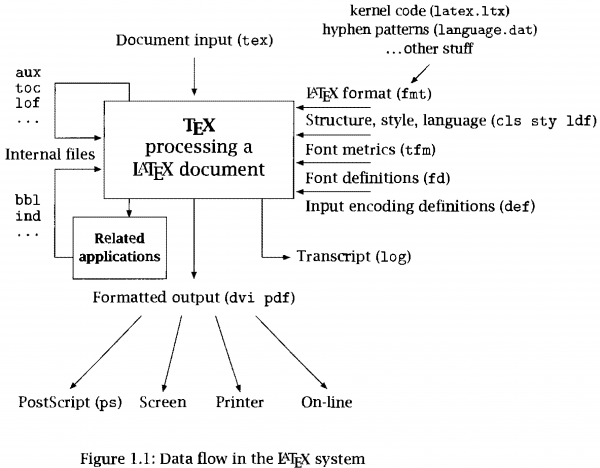
\includegraphics[scale = 0.3]{latex_dataflow.png}
	\caption{\tiny{\LaTeX\ inputs, outputs and supporting files from \href{https://webhost1.ust.hk/~atcwiki/cgi-bin/atcwiki/index.php?title=ATC:LaTeX}{ATC wiki}}}
\end{figure}
\end{frame}

\begin{frame}[fragile]
	\frametitle{The .tex file}
	Most \LaTeX\ documents (including this one) are shaped something like this:
		\begin{semiverbatim}
			\\documentclass[options]\{class\}
			\\usepackage\{package\}
			\\begin\{document\}
			\\tableofcontents
			\\section\{Section Title\}
		\-\	Some content?
		\-\	\$Some maths?\$
			\\end\{document\}
		\end{semiverbatim}
\end{frame}

\begin{frame}
	\frametitle{The .tex preamble (and some other stuff)}
	
	Anything between the \textbackslash documentclass command and the \textbackslash begin\{document\} command is called the preamble. Taken  inclusively, this includes a number of elements.
	
	\begin{description}
		\item[documentclass:] sets automated margins, paper and font size, etc. Chances are you will use a lot of `article' class.
		\item[usepackage:] packages add new options to your document (like libraries). I use grahpicx for include images.
		\item[environments:] make \LaTeX\ use special formatting for figures, tables, lists, images, or maths
	\end{description}
\end{frame}

\begin{frame}[fragile]
	\frametitle{Lists}
	\begin{columns}[T]
		\begin{column}{0.5\textwidth}
				\textbf{Itemized lists:}
			\begin{itemize}
				\item item A
				\item item B
			\end{itemize}	
			\textbf{Enumerated lists:}
			\begin{enumerate}
				\item item AA
				\item item BB
			\end{enumerate}
			\textbf{Description Lists:}
			\begin{description}
				\item[label] item AAA
				\item[label] item BBB
			\end{description}
		\end{column}
		\hspace{-50pt}
		\vrule
		\hspace{30pt}
		\begin{column}{0.5\textwidth}
			\begin{semiverbatim}
				\begin{tiny}
				\\begin\{itemize\}
					\-\ \\item item A
					\-\ \\item item B
				\\end\{itemize\}
				\medskip
				
				\\begin\{enumerate\}
					\-\ \\item item AA
					\-\ \\item item BB
				\\end\{enumerate\}
				\medskip

				\\begin\{description\}
					\-\ \\item[label] item AAA
					\-\ \\item[label] item BBB
				\\end\{description\}
				\end{tiny}
			\end{semiverbatim}
		\end{column}
	\end{columns}
\end{frame}

\begin{frame}[fragile]
	\frametitle{Tables}
	Basic \LaTeX\ tables can be a little unintuitive, but there are some great guidelines for style in the additional resources.\bigskip
	\begin{columns}[c]
		\begin{column}{0.45\textwidth}
		\begin{tabular}{| l l l |}
			\hline
			Column 1 & Column 2 & Column 3 \\
			\hline \hline
			A & B & C \\
			$\alpha$ & $\beta$ & $\gamma$ \\
			\hline
		\end{tabular}
		\end{column}
		\hspace{30pt}
		\vrule
		\hspace{10pt}
		\begin{column}{0.45\textwidth}
		\begin{semiverbatim}
			\begin{tiny}
				\\begin\{tabular\}\{\textbar l l l \textbar\}
					\\hline
					Column 1 \& Column 2 \& Column 3 \\\\
					\\hline \\hline
					A \& B \& C \\ \\\
					\$\\alpha\$ \& \$\\beta\$ \& \$\\gamma\$ \\\\
					\\hline
				\\end\{tabular\}
			\end{tiny}
		\end{semiverbatim}
		\end{column}
	\end{columns}
\end{frame}

\begin{frame}[fragile]
	\frametitle{Images}
	\begin{columns}[c]
		\begin{column}{0.5\textwidth}
			\hspace{10pt}
		\begin{figure}
			\begin{centering}
			
\includegraphics[scale=0.25]{enjoy_science.jpg}
			\label{enjoy_science}
			\caption{Enjoy Science!}
			\end{centering}
		\end{figure}
		\end{column}
	\hspace{30pt}
	\vrule
	\hspace{10pt}
		\begin{column}{0.5\textwidth}
			\begin{tiny}
		\begin{semiverbatim}
				\\begin\{figure\}
					\\begin\{centering\}
						\\includegraphics[scale=0.25]\{enjoy\_science.jpg\}
						\\label\{enjoy\_science\}
						\\caption\{Enjoy Science!\}
					\\end{centering}
				\\end\{figure\}
		\end{semiverbatim}
					\end{tiny}
		\end{column}
	\end{columns}
	\begin{centering}
	\tiny{image courtesy of: \href{https://scientiasalon.wordpress.com/2014/08/25/science-is-not-a-frog/}{Scientia Salon}}
	\end{centering}
\end{frame}

\begin{frame}
	\frametitle{Writing Math 1}
	
	Math mode is called between \$ symbols. There are two kinds of math modes. In inline math mode(\$math\$), math appears like this: $f(x)= \sum_n{i=0}^{n} \frac{(a_i)}{1 + x}$ In display mode (\$\$math\$\$), math appears like this: 	$$f(x)= \sum_n{i=0}^{n} \frac{(a_i)}{1 + x}$$
	
	Notice the difference between the ways that sub/superscript and fractions appear.
	\begin{semiverbatim}
			\$f(x)= \\sum\_n\{i=0\}\^\{n\} \\frac\{(a\_i)\}\{1 + x\}\$
	\end{semiverbatim}
\end{frame}	

\begin{frame}[fragile]
	\frametitle{Writing Math 2}
	Let's take a look at some equations to see how \LaTeX\ handles them! \bigskip
\begin{columns}
	\hspace{-20pt}
	\begin{column}{0.57\textwidth}
		\begin{enumerate}
				\item ${x = \frac{- b \pm \sqrt{b^{2} - 4ac}}{2a} }$
				\item $\oint_C {E \cdot d\ell = - \frac{d}{{dt}}} \int_S {B_n dA}$
				\item $\emptyset = {\{u \in w | (u \in u) \land \lnot(u \in u)}\}$
				\item $\forall x(Px \to Qx)\to\exists o(Po \to Qo)$
		\end{enumerate}
	\end{column}
	\hspace{0pt}
	\begin{column}{0.55\textwidth}
	\begin{enumerate}
		\item {\begin{semiverbatim}\begin{tiny}
\$\{x = \\frac\{- b \\pm \\sqrt\{b^\{2\} - 4ac\}\}\{2a\} \}\$
				\end{tiny} \end{semiverbatim}}
		\item {\begin{semiverbatim}\begin{tiny}
				\$\\oint_C \{E \\cdot d\\ell = - \\frac\{d\}\{\{d\}\}\} \dots 
				\\int_S \{B_n dA\}\$			
				\end{tiny}\end{semiverbatim}}
		\item {\begin{semiverbatim}\begin{tiny}
				\$\\emptyset = \{\\\{u \\in w \textbar (u \\in u) \\land \dots
				\\lnot(u \\in u)\}\}\$			
				\end{tiny}\end{semiverbatim}}	
		\item {\begin{semiverbatim}\begin{tiny}
				\$\\forall x(Px \\to Qx)\\to\\exists o(Po \\to Qo)\$			
				\end{tiny}\end{semiverbatim}}
	\end{enumerate}
	\end{column}
\end{columns}
\end{frame}


%------------------------------------------------
\section{Learning \LaTeX}
%------------------------------------------------

\begin{frame}
\frametitle{What tools are available to me?}
\begin{columns}
	\begin{column}{0.5\textwidth}
Edittor/Compilers:
\begin{itemize}
	\item {\TeX Shop}
	\item {\TeX Studio}
	\item {Overleaf (Online)}
	\item {Share\LaTeX\ (Online)}
\end{itemize}
\end{column}
\begin{column}{0.5\textwidth}
	Distributions:
\begin{itemize}
	\item MiK\TeX
	\item \TeX Live
	\item Max\TeX
\end{itemize}
\end{column}
\end{columns}
Or write \LaTeX\ in your emacs :p
\end{frame}

\begin{frame}
\frametitle{Resources}
\begin{itemize}
	\item{\href{https://www.inf.ethz.ch/personal/markusp/teaching/guides/guide-tables.pdf} {P\" uschel's {\em Small Guide to Making Nice Tables}}}
	\item{\href{tex.stackexchange.com}{tex.stackexchange.com}}
	\item{Googling `Introduction to \LaTeX'}
	\item{\href{http://texdoc.net/texmf-dist/doc/plain/gentle/gentle.pdf}{Michael Doob's {\em Gentle Introduction to} \TeX}}
\end{itemize}
\end{frame}

\end{document}
